\section{Experimentación}

\subsection{Caso de estudio: Red laboral}

Antes de analizar la captura sosteníamos como hipótesis que la topología de los mensajes ``tendría forma de árbol'' con el router en su raíz y tantas hojas como hosts dentro de la red, con poco o nada de interacción entre ellos.\newline

También suponíamos que la mayoría de las redes \textit{subneteadas} con un router tendrían necesariamente esta forma.\newline

En este caso estudiamos la red de una oficina con alrededor de 40 computadoras y teléfonos celulares.\newline

La captura duró alrededor de seis horas con más de 90000 mensajes ARP who-has. Con este volumen de datos fue necesario seccionar el análisis bajo diferentes criterios, como la cantidad de mensajes o una cantidad mínima de mensajes entre nodos.\newline

Los grafos presentados a continuación muestran direcciones IP como nodos unidos por un eje si el nodo origen realizó un broadcast ARP who-has buscando al nodo destino.\newline

Para empezar, mostramos los primeros 10 mil requests entre los nodos que se enviaron diez o más mensajes. Elegimos esta parte de la muestra tras haber visto que graficar más nodos agrega poca información nueva respecto de los nodos más relevantes.\newline

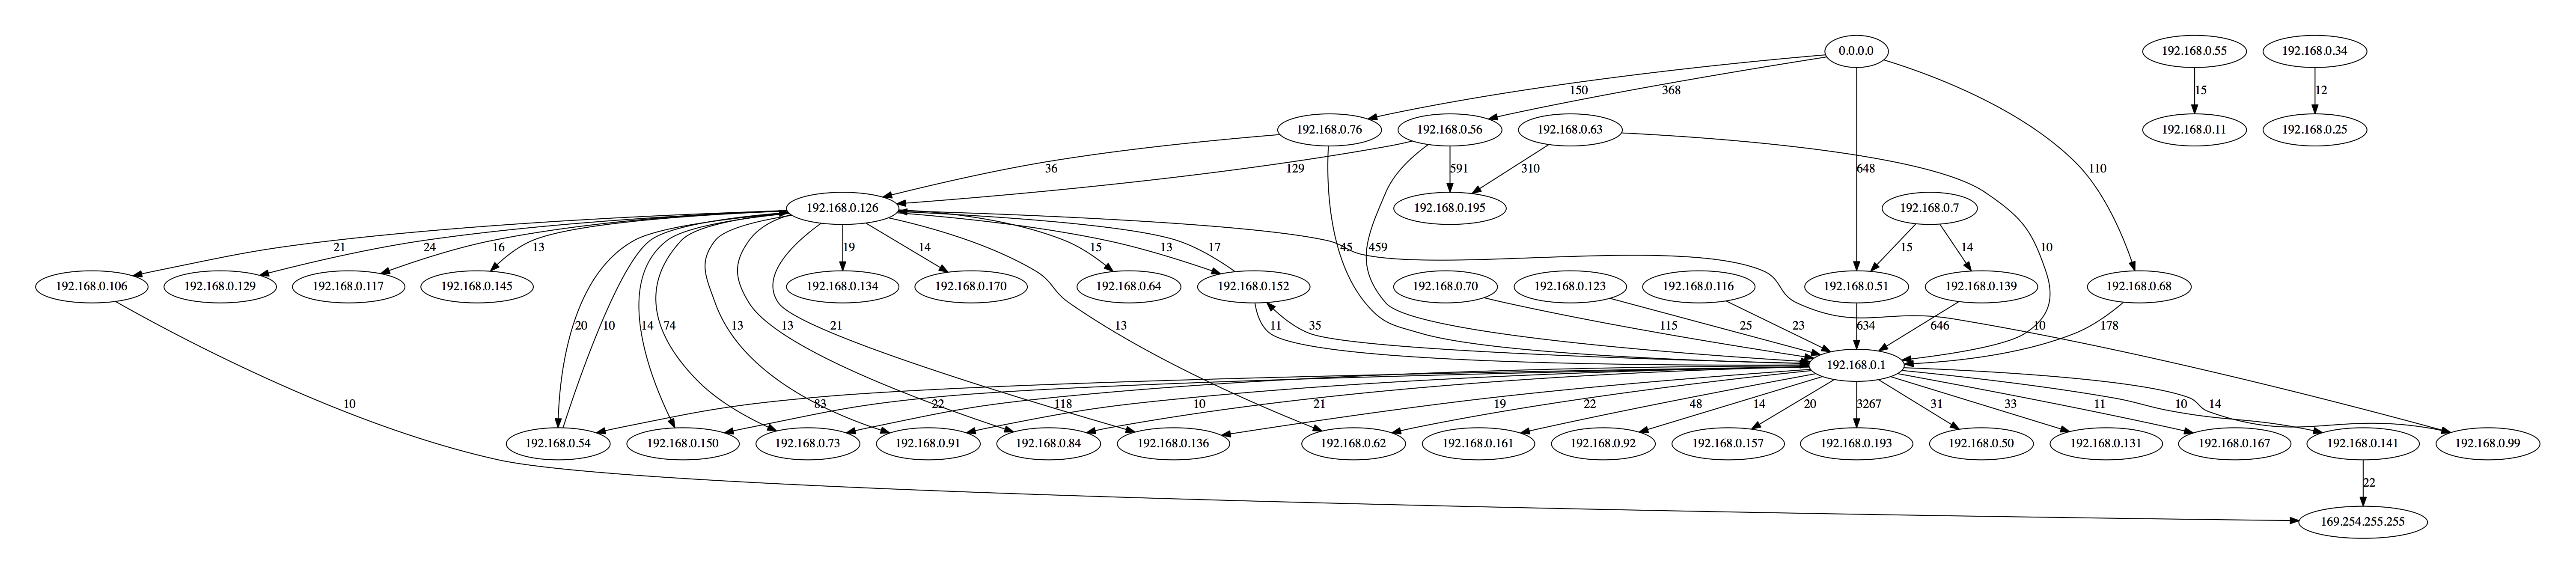
\includegraphics[scale=0.25,angle=90]{graphics/t-work-10000c-10w.png}

A primera vista notamos que hay ciertos nodos que resaltan sobre los demás como el 192.168.0.1 (router), o 192.168.0.126. Si bien la estructura de este digrafo no es un árbol, se nota que hay cierta jerarquía.\newline

Un nodo interesante que resalta es el 169.254.255.255, porque es la única IP no privada que aparece en la red. Analizando este caso en particular, vemos que siempre es buscado por nodos de la red (y éste nunca busca a nadie), lo que nos hace suponer que puede tratarse de un servicio, como un servidor de DNS.\newline

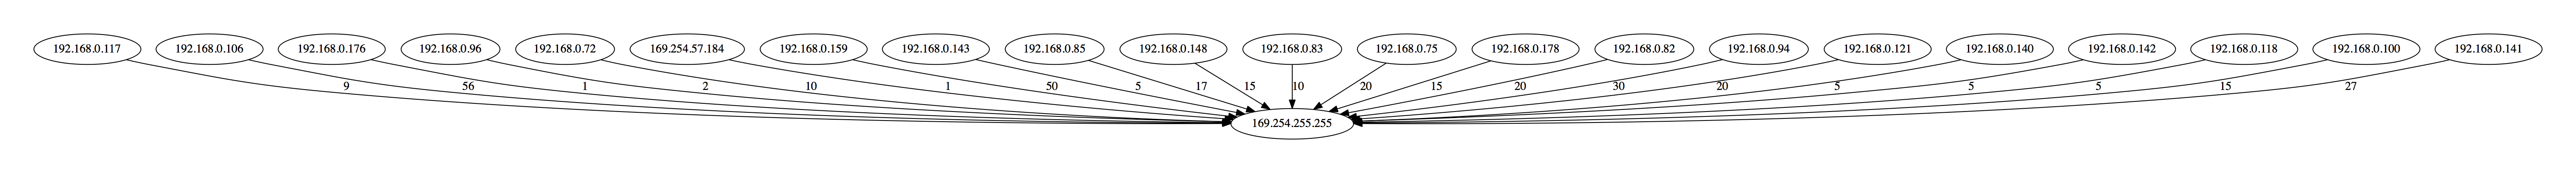
\includegraphics[scale=0.25,clip=true,trim=850 0 870 0]{graphics/t-work-ip-169-254-255-255.png}

Investigando el resto de la captura, notamos que los demás paquetes que recibe son del protocolo NetBIOS Name Service, con lo que podemos afirmar que en este nodo funciona un NetBIOS Server.\newline

Para poder reconocer mejor cuáles son los nodos más importantes de la red veamos el siguiente grafo, donde se estudia toda la muestra pero sólo nos quedamos con aquellos nodos que compartieron más de mil mensajes.\newline

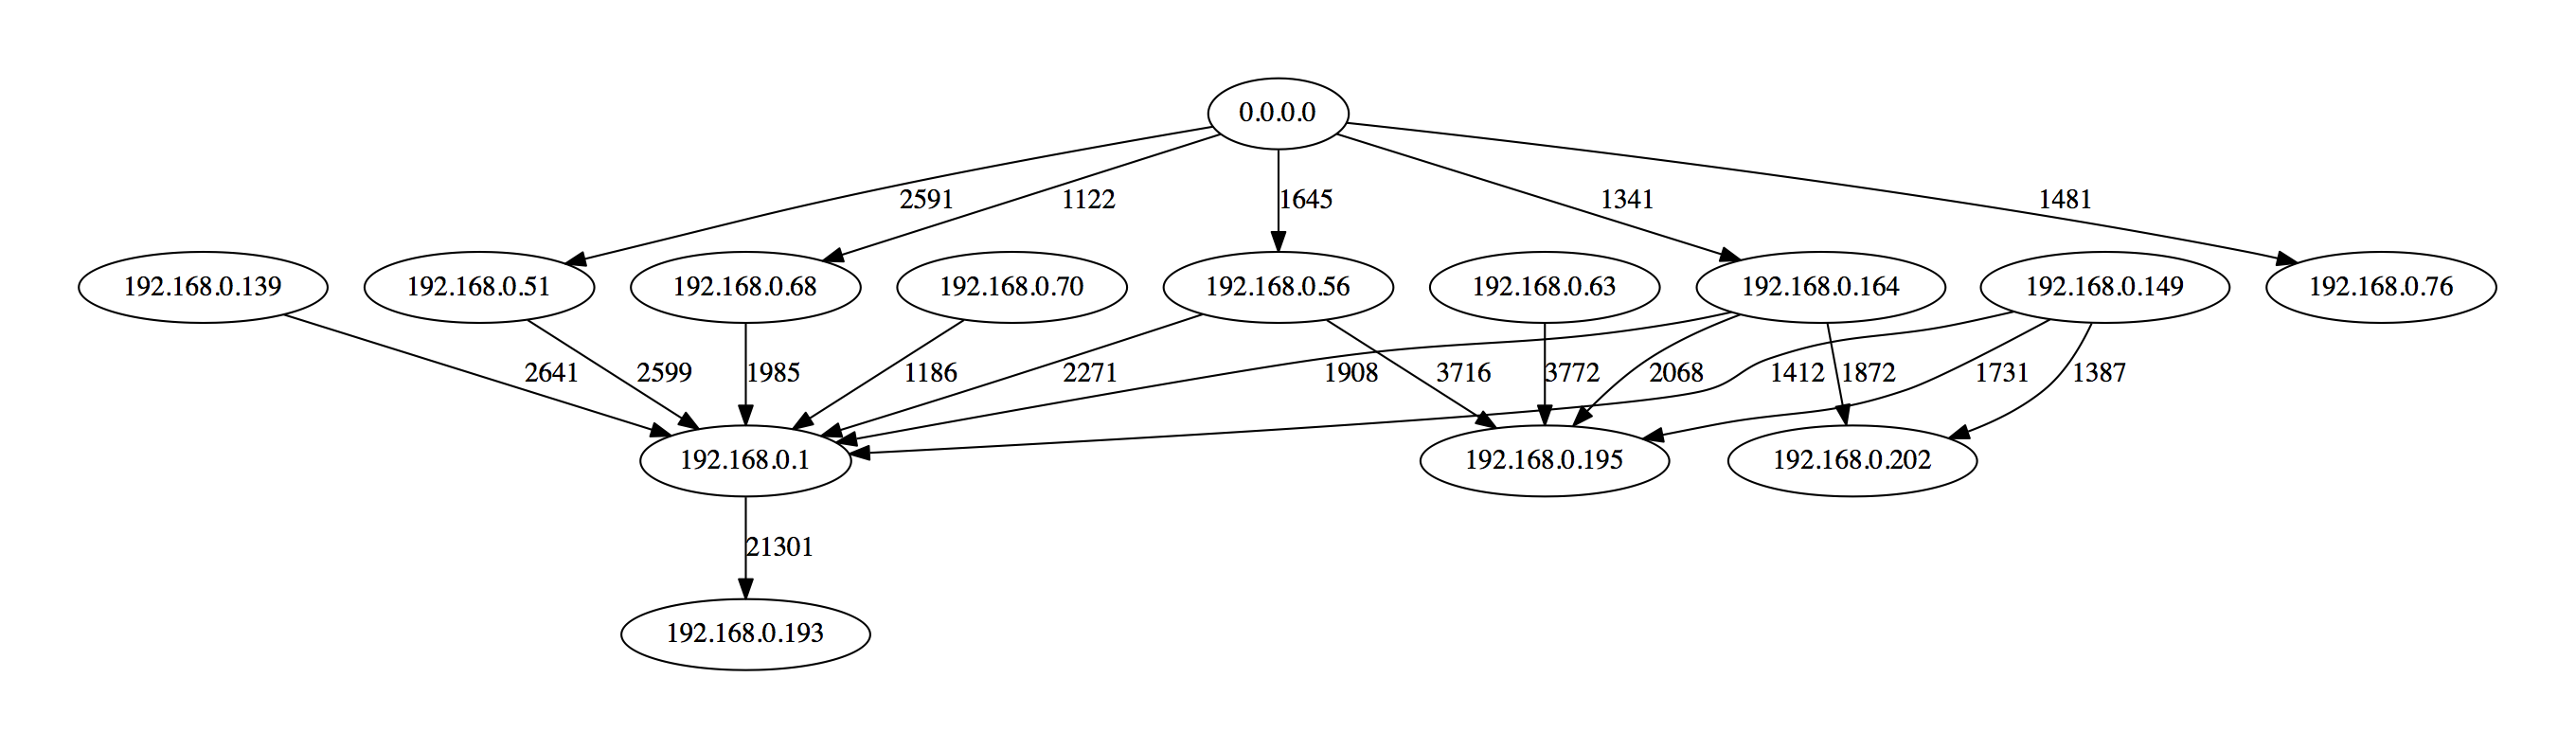
\includegraphics[scale=0.30]{graphics/t-work-all-1000w.png}

Viendo los mensajes ARP de esta manera podemos notar varias cosas. Por un lado que tiene forma de árbol, pero el nodo raíz no es el router, como suponíamos originalmente. Vemos que hay muchos requests ARP que tienen origen en el 0.0.0.0 y como destino diversos nodos de la red, pero ésta no es una IP del rango privado.\newline

Este primer hecho nos llevó a conocer que un ARP con origen 0.0.0.0 es parte de una técnica para detectar direcciones IP duplicadas dentro de una red. En este caso, se estaba queriendo detectar si las direcciones terminadas en 51, 56, 68, 76 ó 164 estaban duplicadas.\newline

\newpage

También nos pareció relevante analizar el router en particular.\newline

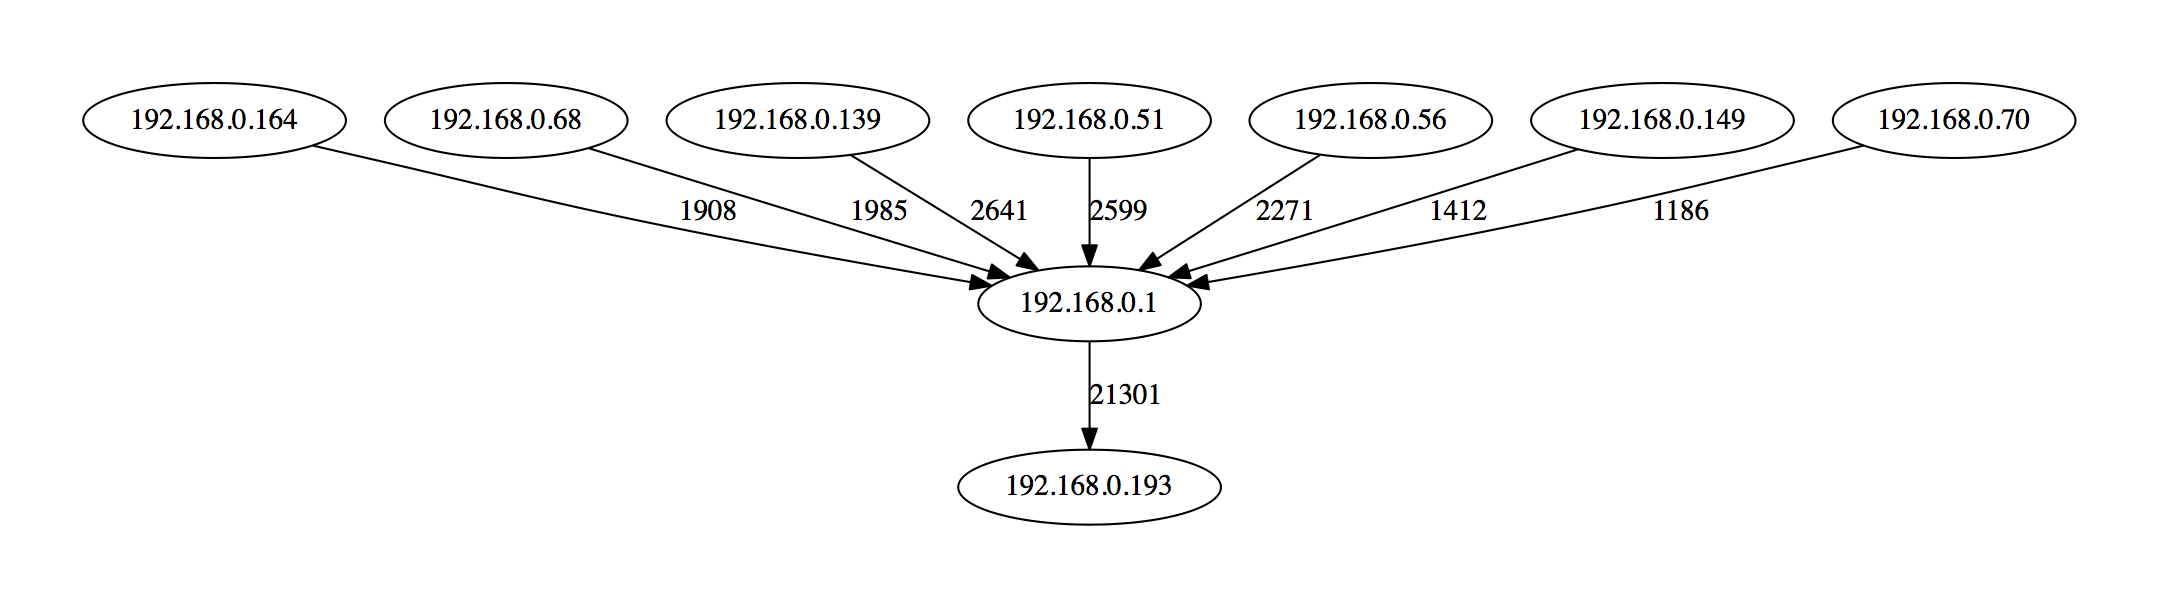
\includegraphics[scale=0.3]{graphics/t-work-router-1000w.png}

Vemos que resulta interesante la gran cantidad de veces que se solicita la IP 192.168.0.193. Para saber más sobre lo que podría estar sucediendo con ese host, revisamos el resto de la captura pero encontramos que no había ningún paquete con esa dirección origen ni destino.\newline

Por esto creemos que podría tratarse de un nodo mal configurado, buscando una IP que ya no existe en la red, lo cual parece en consonancia con la gran cantidad de pedidos ARP que el router le hace.\newline

Finalmente, calculamos la entropía de las fuentes origen y destino: 3.44356252078915 y 4.652923252101102, respectivamente.\newline


\subsection{Caso de estudio: Otra red laboral}

\indent \indent  En este segundo caso de estudio, se estudió la red de las oficinas donde trabaja otro de los integrantes del grupo. La captura de datos se realizó por el lapso de dos horas, en modo promiscuo y en un host conectado por cable Ethernet a la red, en contraposición con el caso anterior.\\
\indent Dada la enorme cantidad de datos y, además, para analizar un poco la progresión de la captura, se consideraron tres casos.\\
\indent El primer caso corresponde a los primeros mil paquetes ARP who-has que se capturaron, y nos servirá como primera aproximación. Como caso intermedio, estudiamos luego los primeros seis mil paquetes ARP who-has, que se corresponden aproximadamente con la mitad de los paquetes de dicho tipo capturados a lo largo del experimento. Finalmente, se estudió el caso con todos los paquetes ARP who-has capturados.\\
\indent En los tres casos se calcularon las entropías de las fuentes \textit{Fuente} y \textit{Destino}, y además se proveen histogramas que muestran las direcciones IP que mayor cantidad de pedidos hicieron y las que más fueron pedidas respectivamente. Sin embargo, hemos de aclarar que, para facilitar la visualización, en dichos histogramas se ignoran arbitrariamente IPs que no cumplen con cierta cantidad de apariciones en cada fuente, pudiendo de esta manera analizar más concisamente dichas IP.\\
\indent Es oportuno mencionar también que se proveen grafos dirigidos donde el nodo origen corresponde a la IP que pidió a la IP representada por el nodo destino para los primeros dos subcasos de estudio, pero no para el tercero. La sencilla razón es que la gran cantidad de nodos provoca que el grafo sea, a efectos prácticos, ilegible.\\
\indent Sobre los histogramas deseamos hacer un comentario más: si bien los calculamos basados en la cantidad de apariciones de la IP en la correspondiente fuente, es claro que dado lo mencionado en la introducción acerca de que un evento con mayor probabilidad provee menos información, los gráficos que hicimos inducen lo mismo que si en el eje \textit{y} considerásemos el valor numérico de la información de la IP, aunque en ese caso, los histogramas serían \textit{al revés}, en el sentido de que las IP's que aparecen con barras pequeñas en nuestros gráficos lo harían con barras grandes si midiésemos por la infomación que suministra.\\

\subsubsection{Primeros mil paquetes ARP who-has (Muestra chica)}

\indent \indent Analizando las direcciones IPs que más pedidos hicieron, se obtuvo el siguiente histograma, que representa a las IP's en función de la cantidad de apariciones.

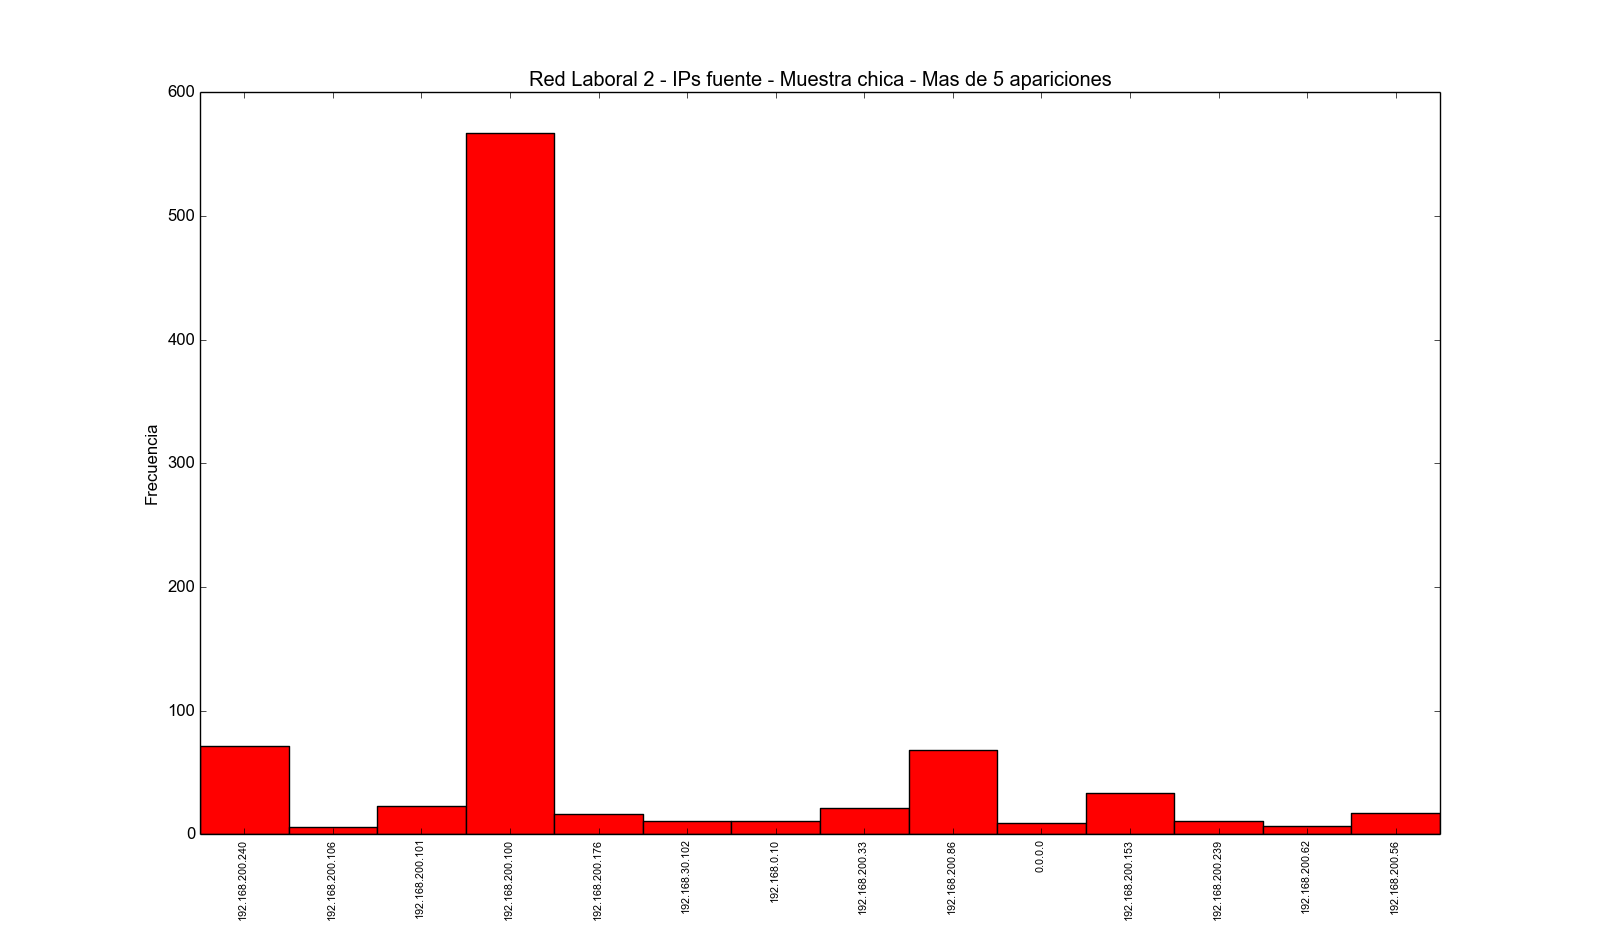
\includegraphics[scale=0.5,clip=true,trim=140 0 0 0]{graphics/laburochico_src.png}


\indent Es de notar que para el gráfico anterior se consideraron IP's con más de cinco pedidos\ realizados. Se observa claramente que la IP 192.168.200.100 realiza la mayor cantidad de pedidos, seguido de lejos por las direcciones 192.168.200.240 y la 192.168.200.86. Se extrae de aquí, entonces, que estas IP's son los símbolos que menor valor aportan a la entropía de la fuente.\\

\indent Para la fuente destino, se obtuvo el siguiente histograma:

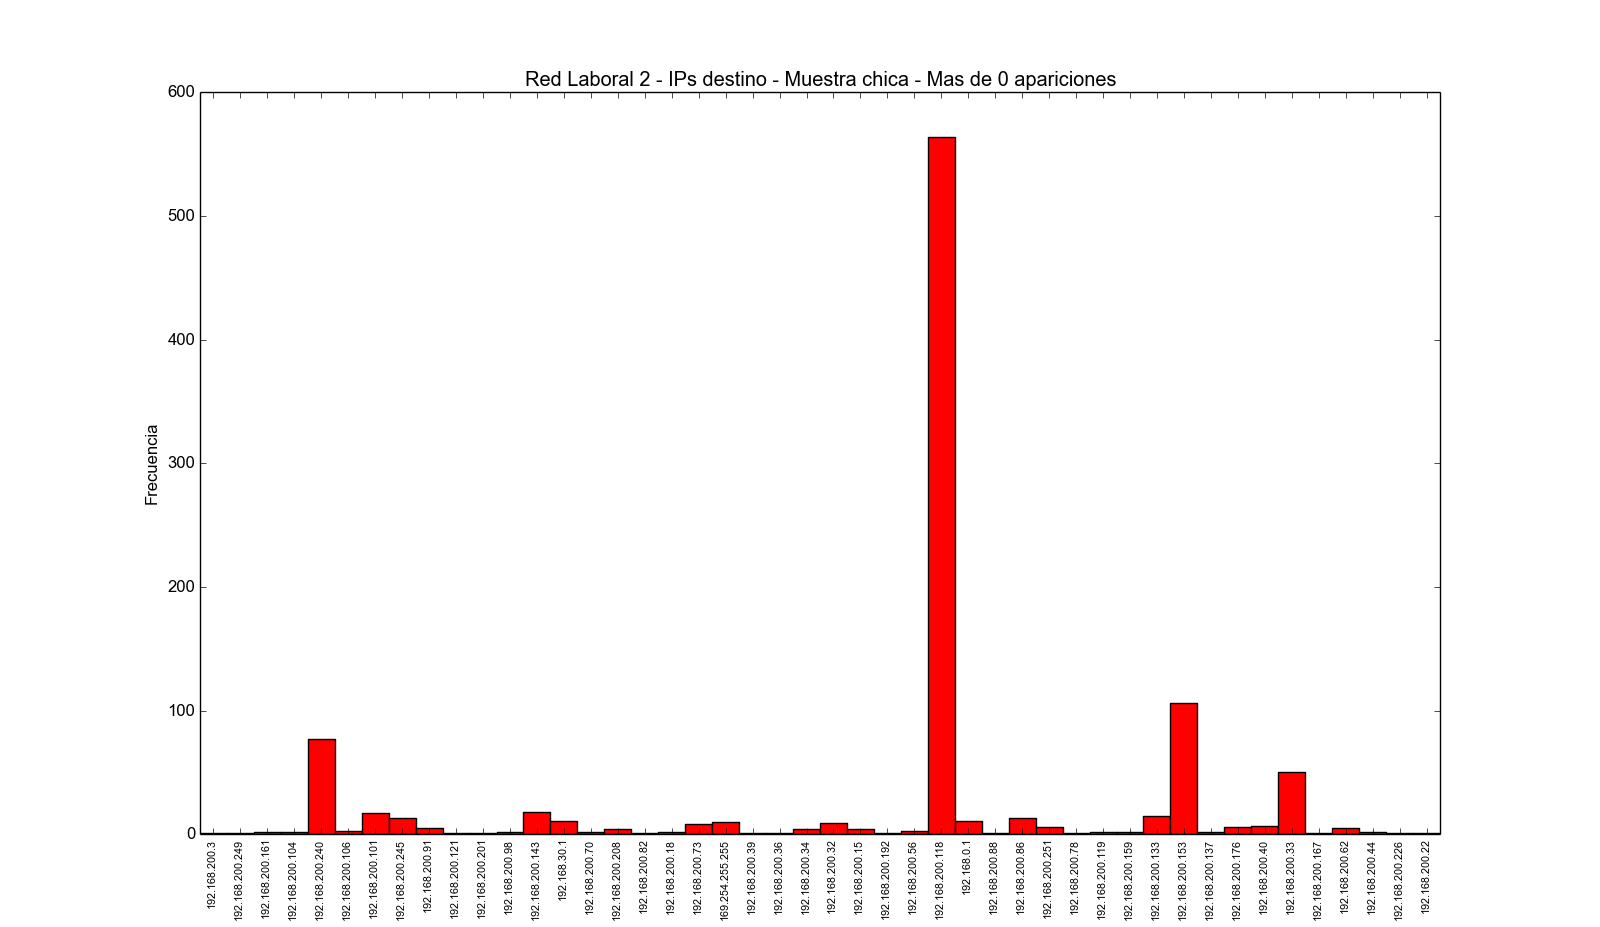
\includegraphics[scale=0.5,clip=true,trim=140 0 0 0]{graphics/laburochico_dst.png}


\indent Aquí se observa que los símbolos que son más pedidos y que por lo tanto menos aportan al valor de la entropía de la fuente destino son, principalmente, la dirección 192.168.200.118 seguido de lejos por la 192.168.200.153 y finalmente la 192.168.200.240. Estas dos últimas direcciones serán más relevantes a medida que se aumentan la cantida de paquetes en consideración. Es notable además que en el anterior gráfico se consideraron todas las IP's que aparieron como destino en los paquetes ARP who-has.\\

\indent A continuación se provee el grafo que se obtuvo para esto subcaso de estudio:\\

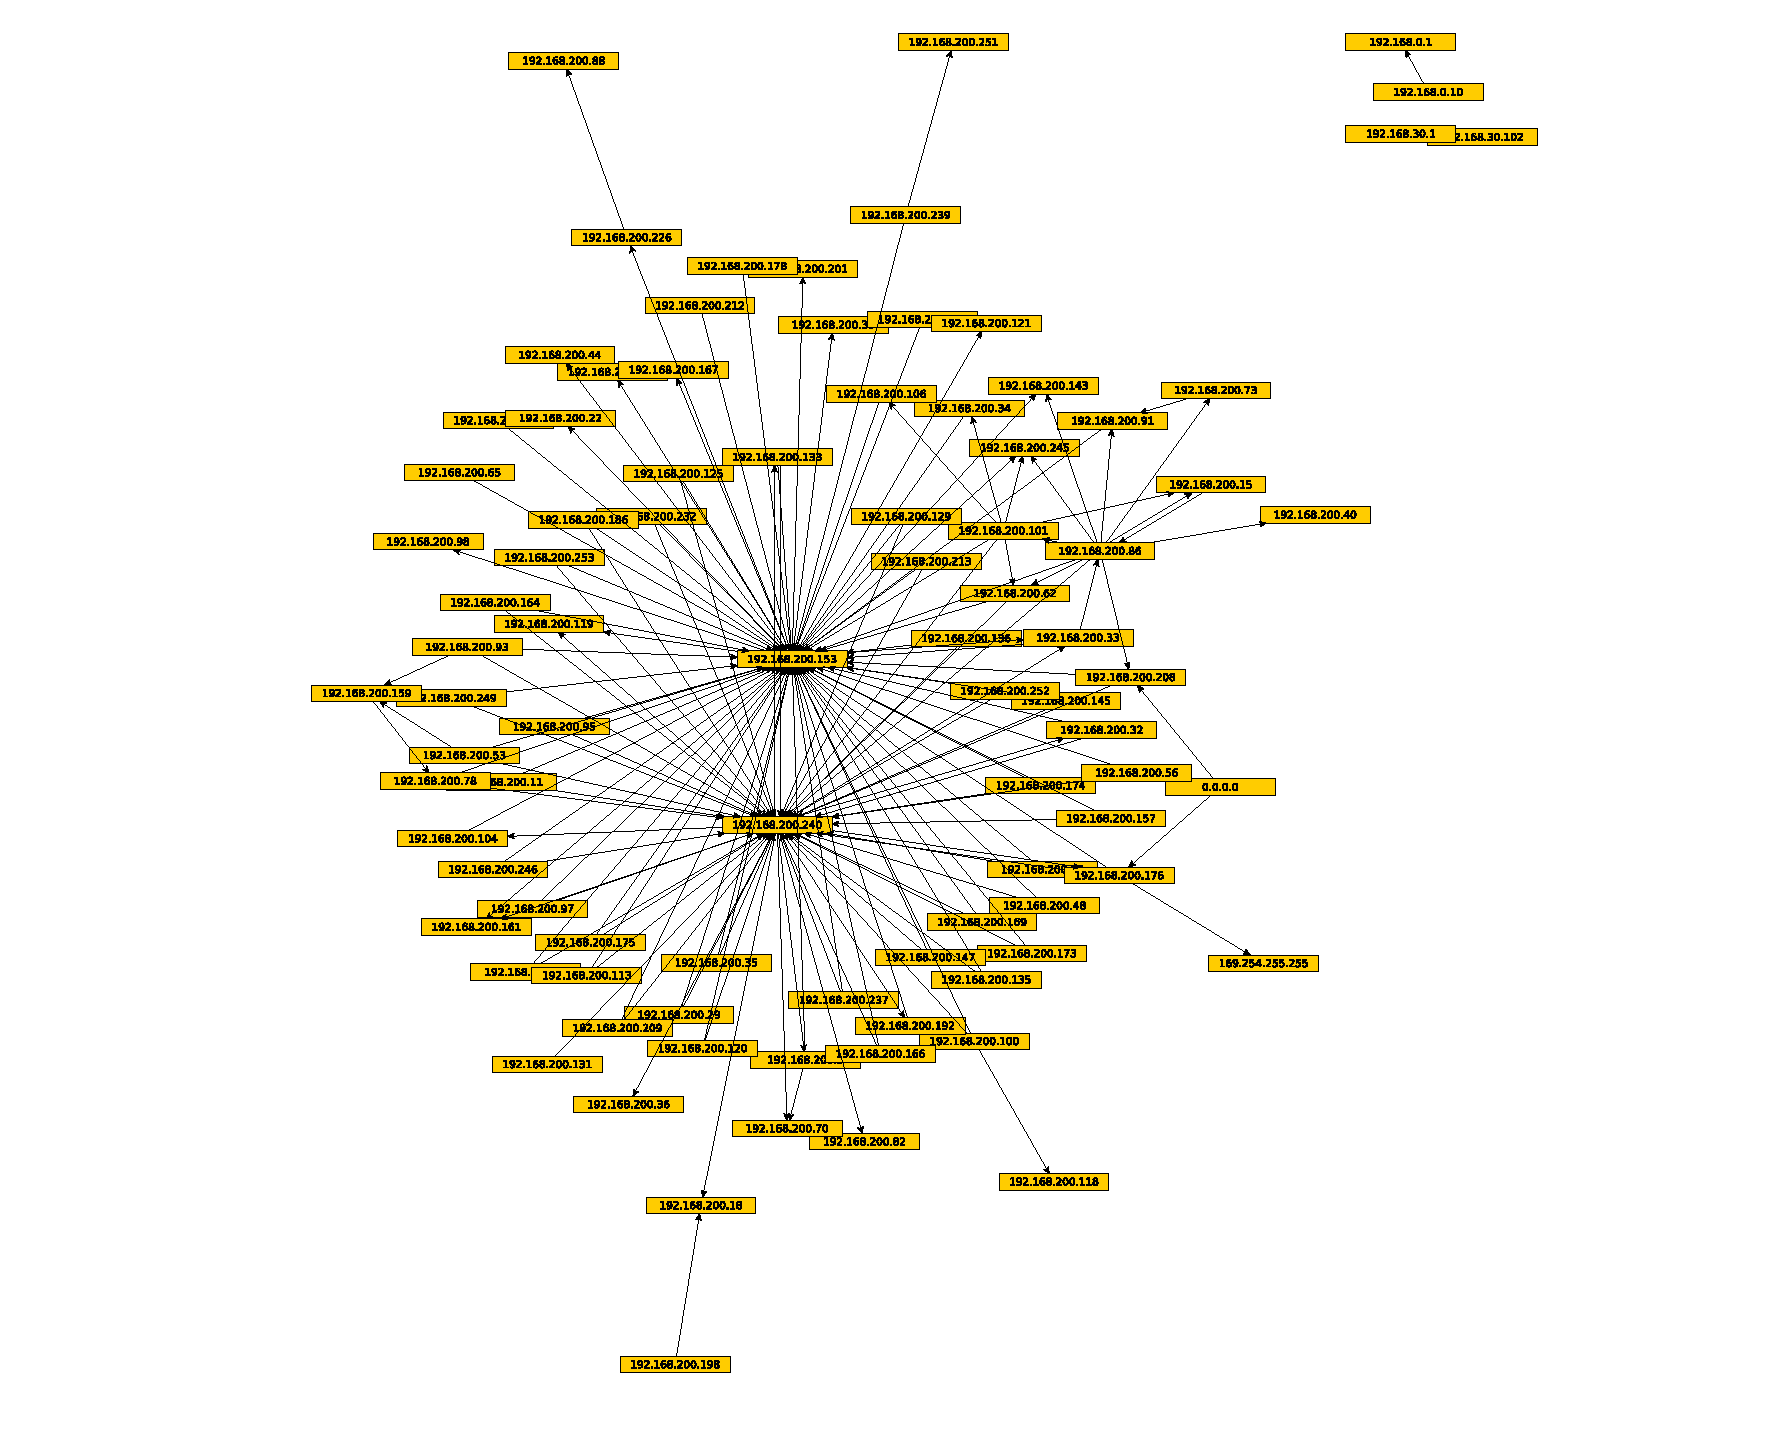
\includegraphics[scale=0.7,clip=true,trim=140 0 0 0]{graphics/laburochico.pdf}


\indent Dado que el grafo no posee peso en sus aristas pero analizándolo en conjunción con los histogramas anteriores, se puede observar que aunque la dirección 192.168.200.118 fue la más pedida en cantidad de pedidos totales, las IP's 192.168.200.240 y 192.168.200.153 fueron pedidas por una mayor cantidad de host distintos, por lo cual creemos que tienen más relevancia en la red.\\

\indent Finalmente las entropías que se calcularon para las fuentes {$S_{src}$} y $S_{dst}$ son:\\

\begin{centering}
	\begin{tabular}{ | c | c | c |} \hline
	   & \textbf{$S_{src}$} & \textbf{$S_{dst}$} \\ \hline
	  	\textbf{Entropía} & 3,0752970340992025 bits & 2,746565878682078 bits\\ \hline
	\end{tabular}
\end{centering}


\subsubsection{Primeros seis mil paquetes ARP who-has (Muestra mediana)}

\indent \indent Análogamente al subcaso anterior, mostramos los gráficos que obtuvimos.\\
\indent Para la fuente origen:\\

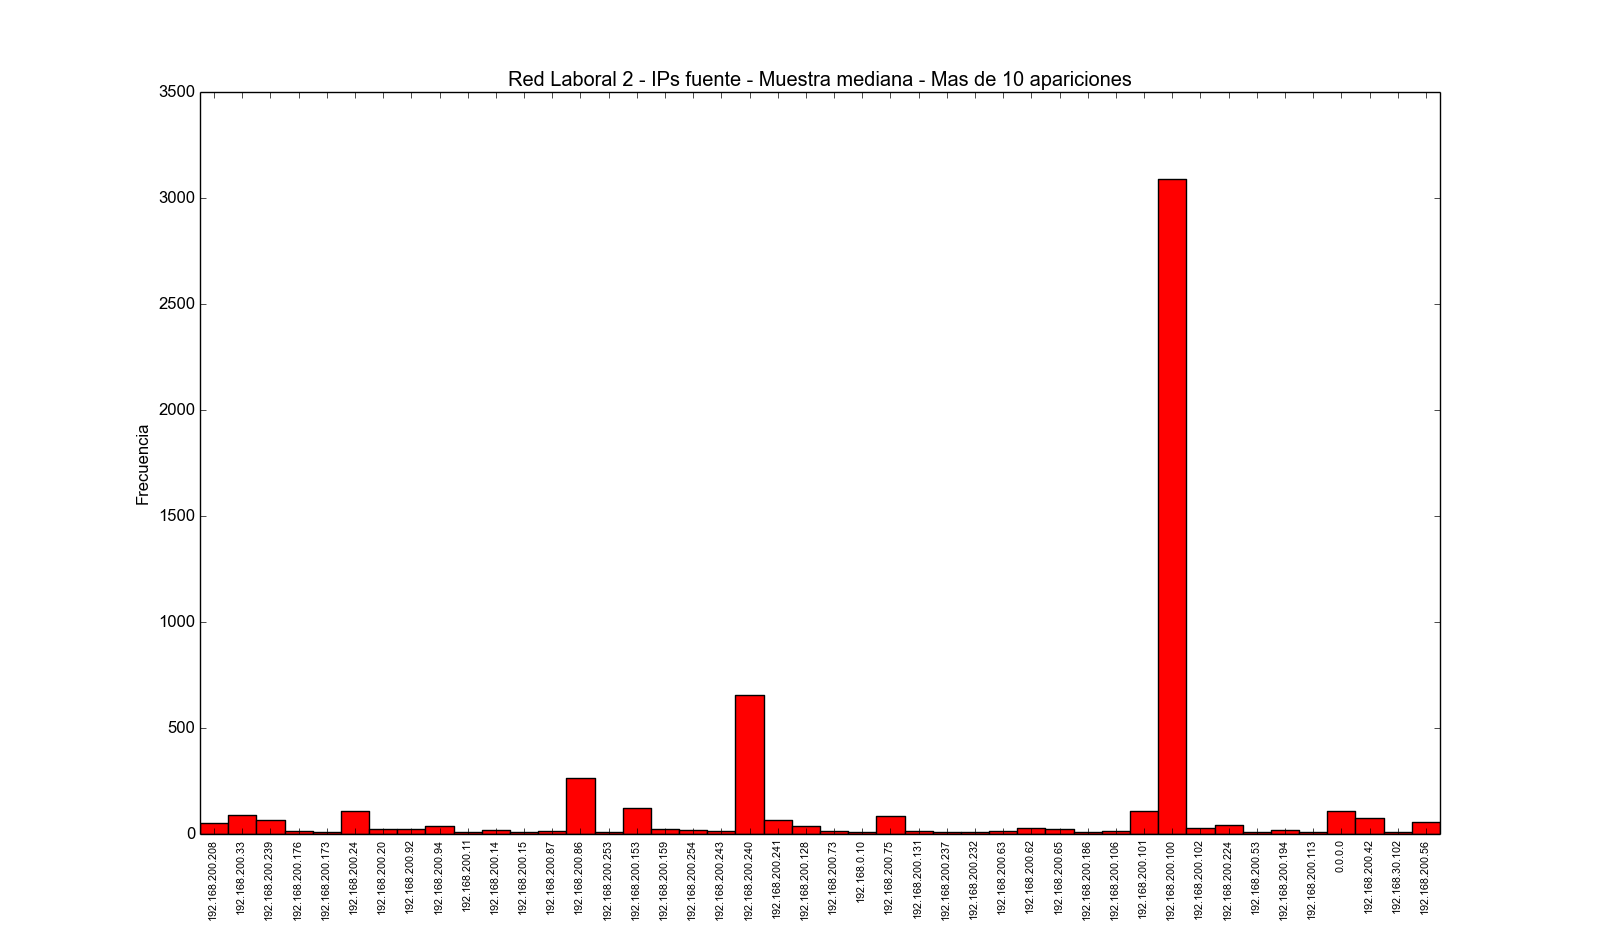
\includegraphics[scale=0.5,clip=true,trim=140 0 0 0]{graphics/laburomediano_src.png}

\indent En este caso se consideraron IP's que realizaron más de 10 peticiones. Aquí sobresale claramente, al igual que en el subcaso anterior, la IP 192.168.200.100, seguida nuevamente por la dirección 192.168.200.240.\\

\indent Sobre la fuente destino:\\

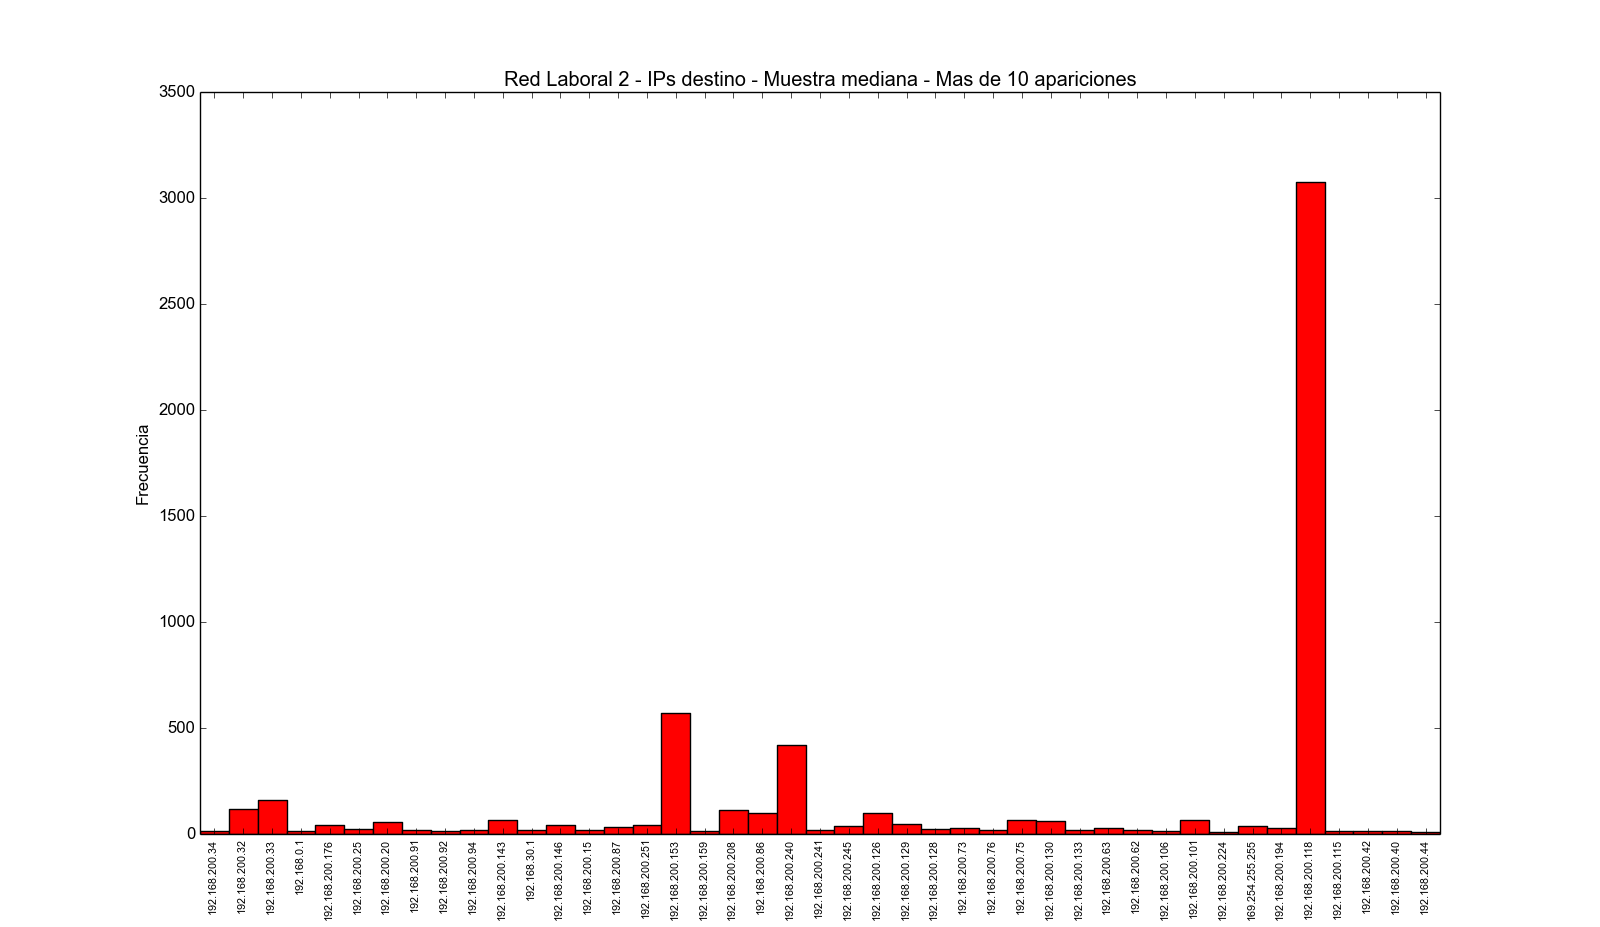
\includegraphics[scale=0.5,clip=true,trim=140 0 0 0]{graphics/laburomediano_dst.png}

\indent  Se observan resultados similares al subcaso de los primeros 1000 paquetes ARP capturados. Aquí ya empezamos a sospechar que la dirección 192.168.200.240 podría tratar se un router o algún artefacto de similares características, puesto que es participe tanto de pedidos como de respuestas.\\

\indent El grafo obtenido:\\

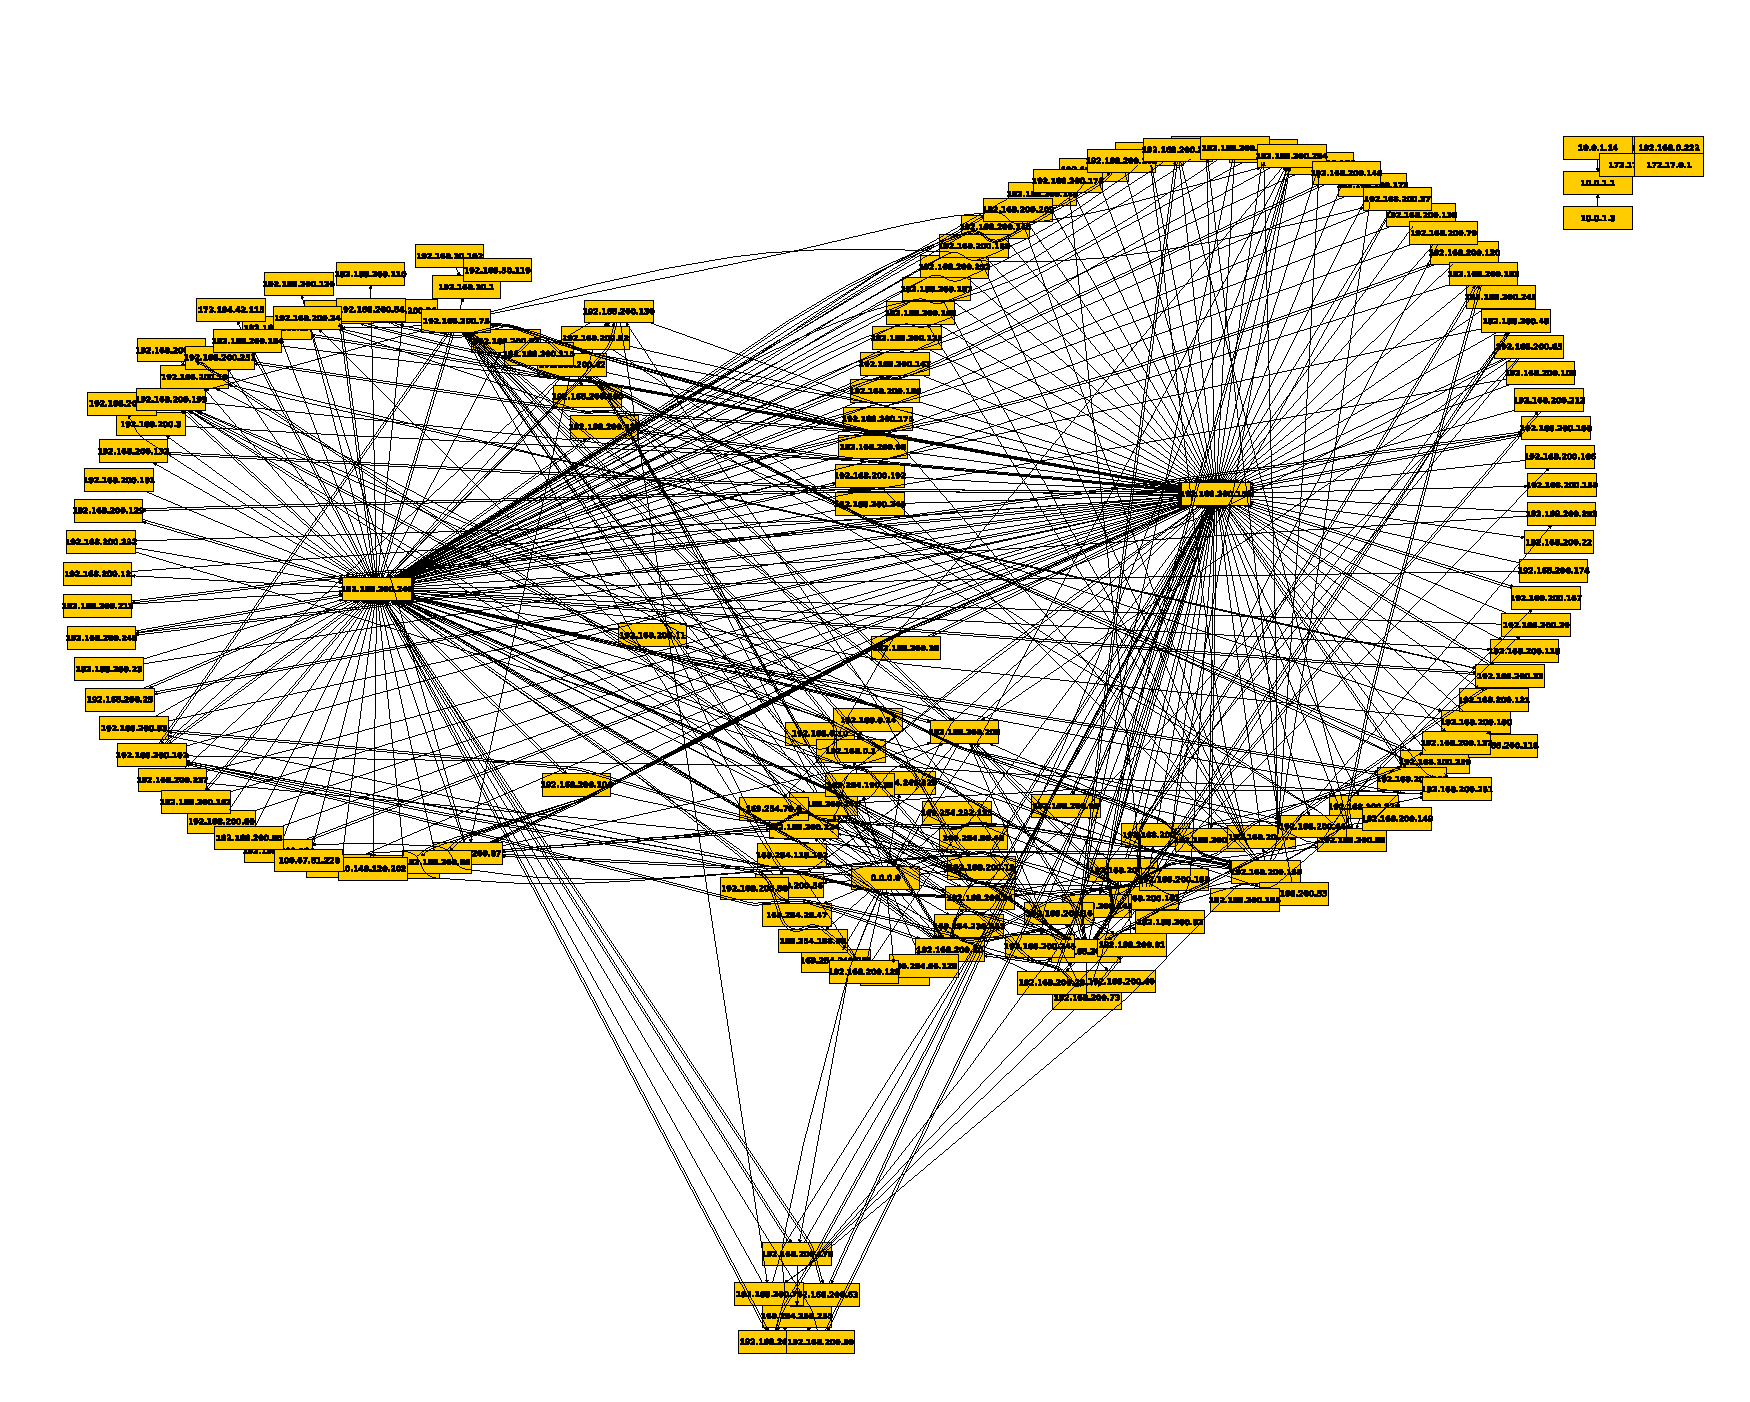
\includegraphics[scale=0.5,clip=true,trim=20 0 0 0]{graphics/laburomediano.pdf}

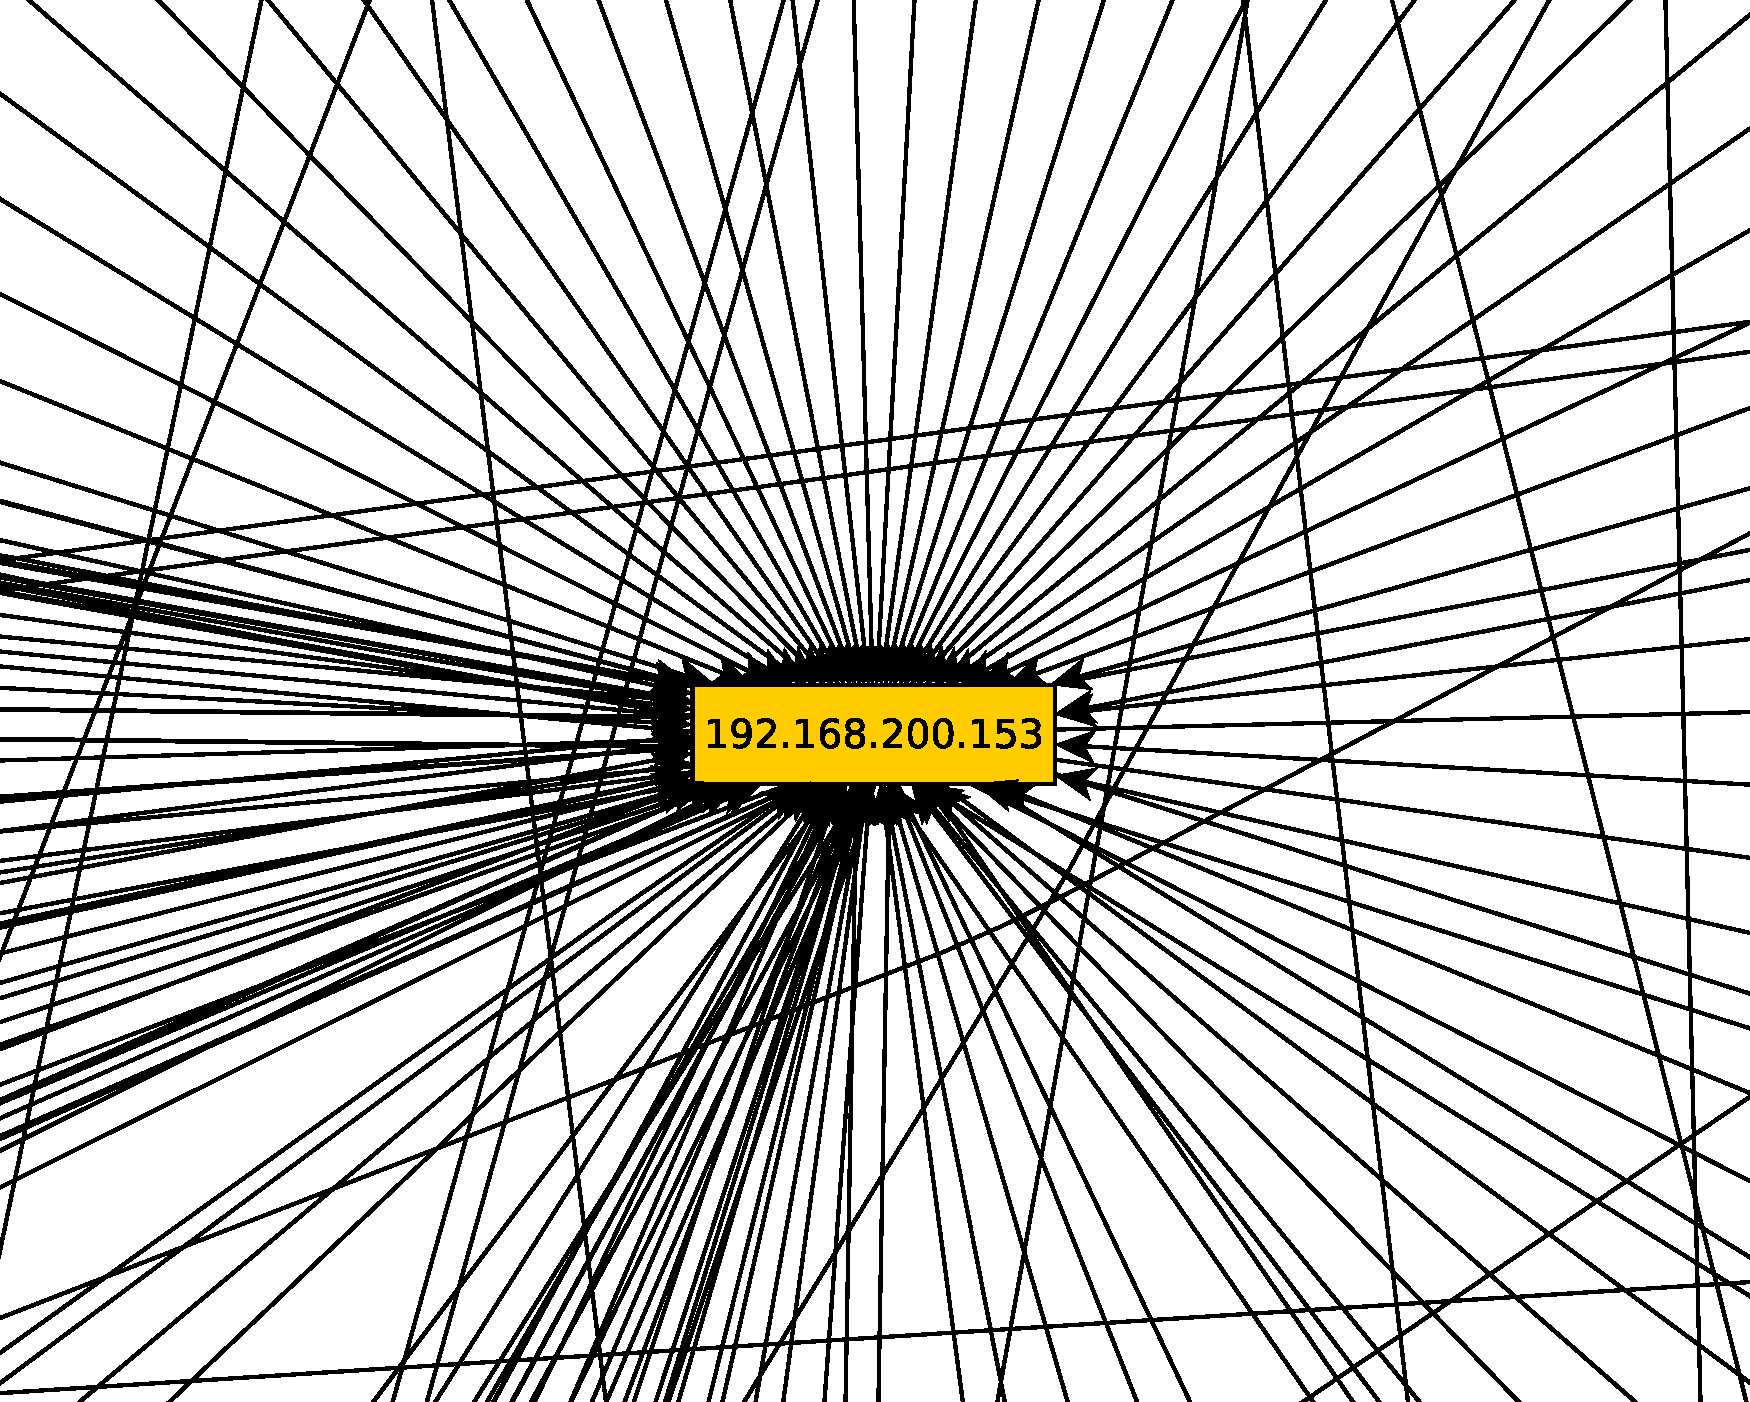
\includegraphics[scale=0.3,clip=true,trim=20 0 0 0]{graphics/laburomediano153.pdf}

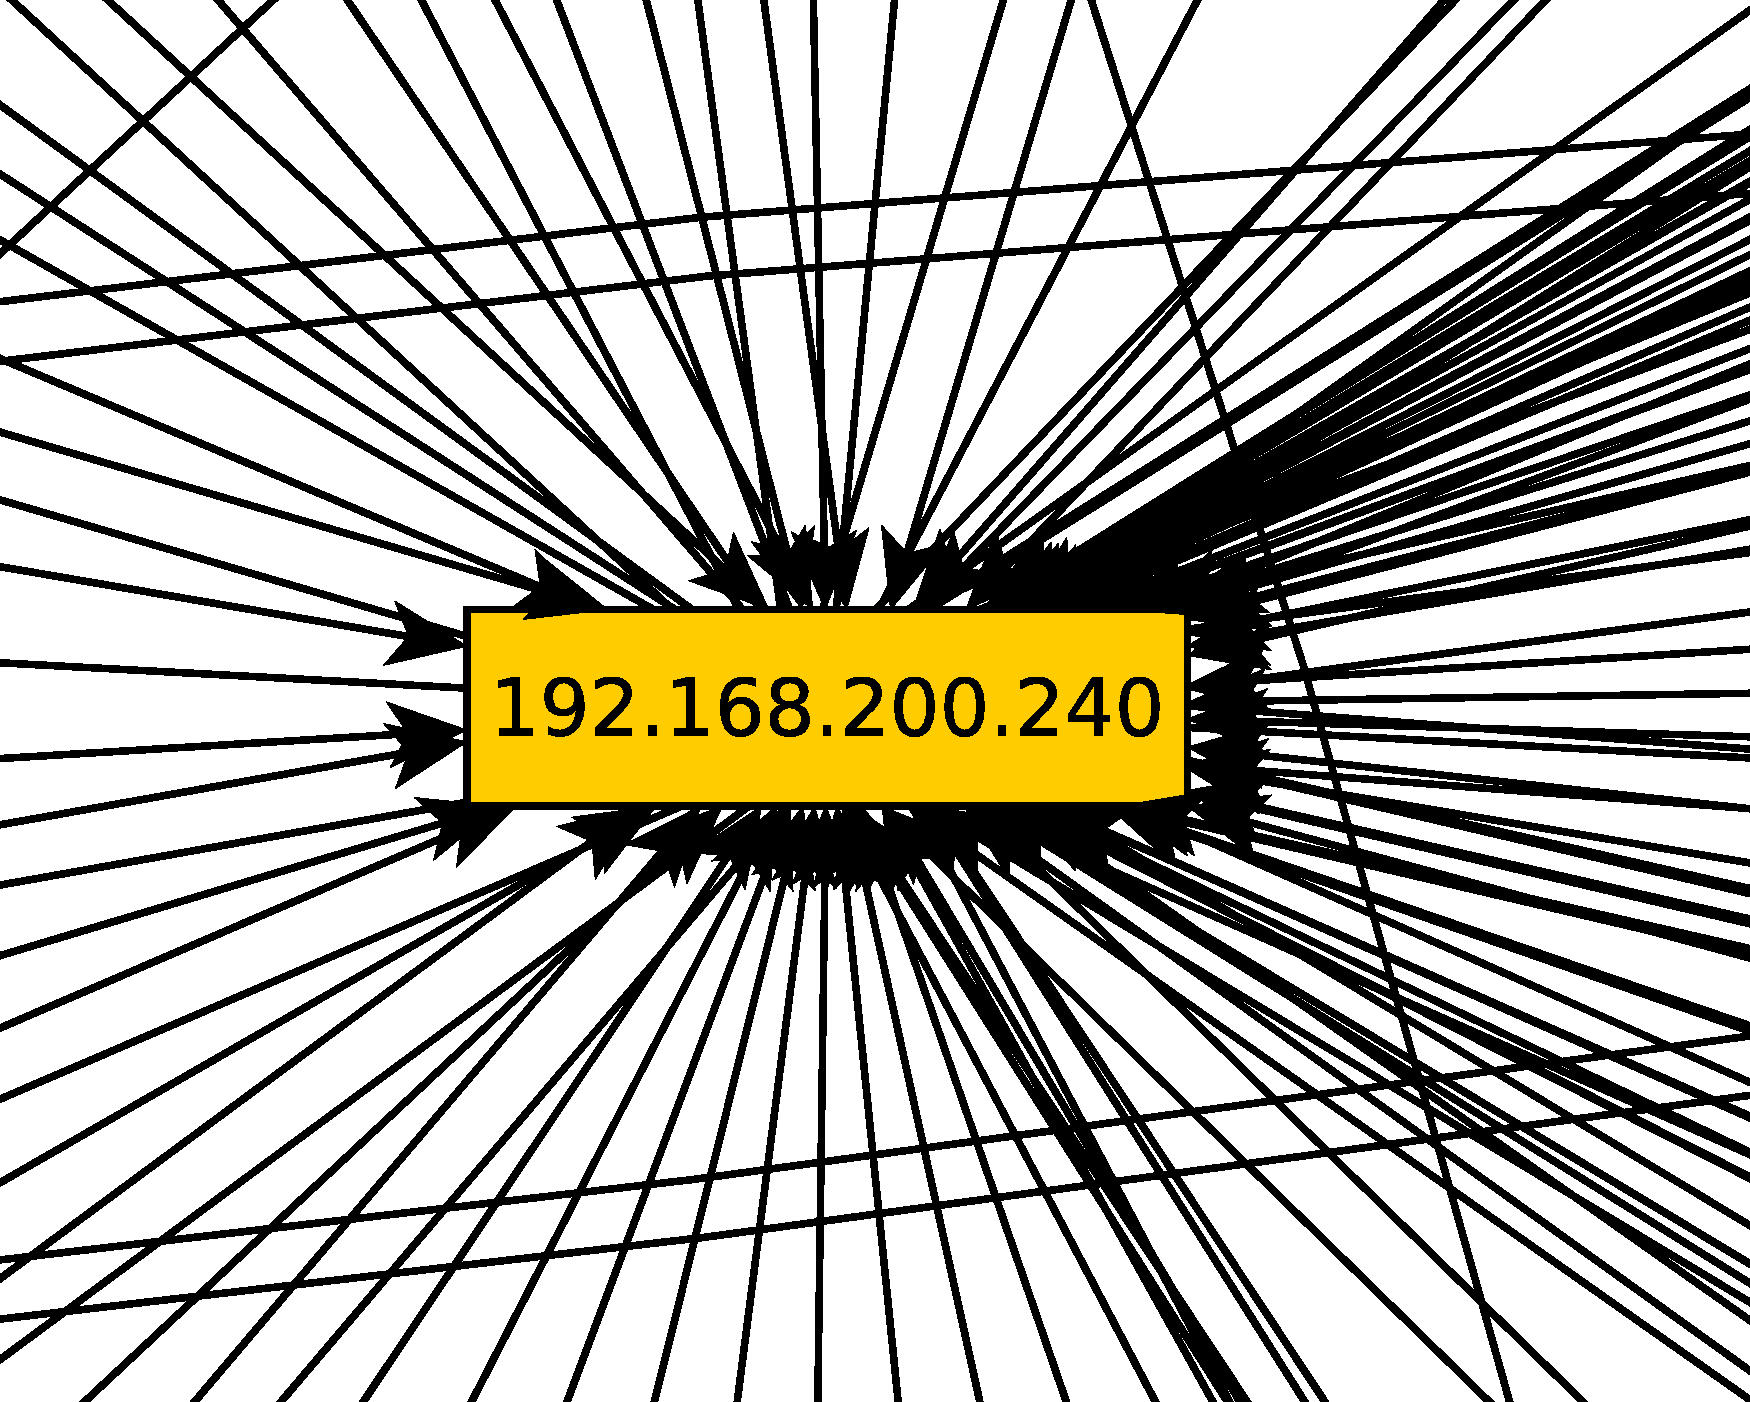
\includegraphics[scale=0.3,clip=true,trim=20 0 0 0]{graphics/laburomediano254.pdf}


\indent Se observan que nuevamente las IP's 192.168.200.240 y 192.168.200.153 son las que son pedidas por mayor cantidad de nodos distintos (a pesar de que la 192.168.200.118 es la que más pedido totales tuvo), aunque en este caso se observa también la IP 0.0.0.0, que como mencionamos anteriormente responde a una técnica que se aplica para detectar direcciones duplicadas.\\

\indent Finalmente, las entropías calculadas:\\

\begin{centering}
	\begin{tabular}{ | c | c | c |} \hline
	   & \textbf{$S_{src}$} & \textbf{$S_{dst}$} \\ \hline
	  	\textbf{Entropía} & 3,535443894743673 bits & 3,434469046688702 bits \\ \hline
	\end{tabular}
\end{centering}\\


\indent Creemos que el aumento en las valores de las entropías se corresponde con el hecho de la aparición de una mayor cantidad de direcciones IP's, que al aparecer en pocas oportunidades en las fuentes proveen más información.\\


\subsubsection{Todos los paquetes ARP who-has capturados (Muestra grande)}

\indent \indent Al igual que en los dos subcasos anteriores, exponemos los gráficos que obtuvimos.\\
\indent Para la fuente origen:\\


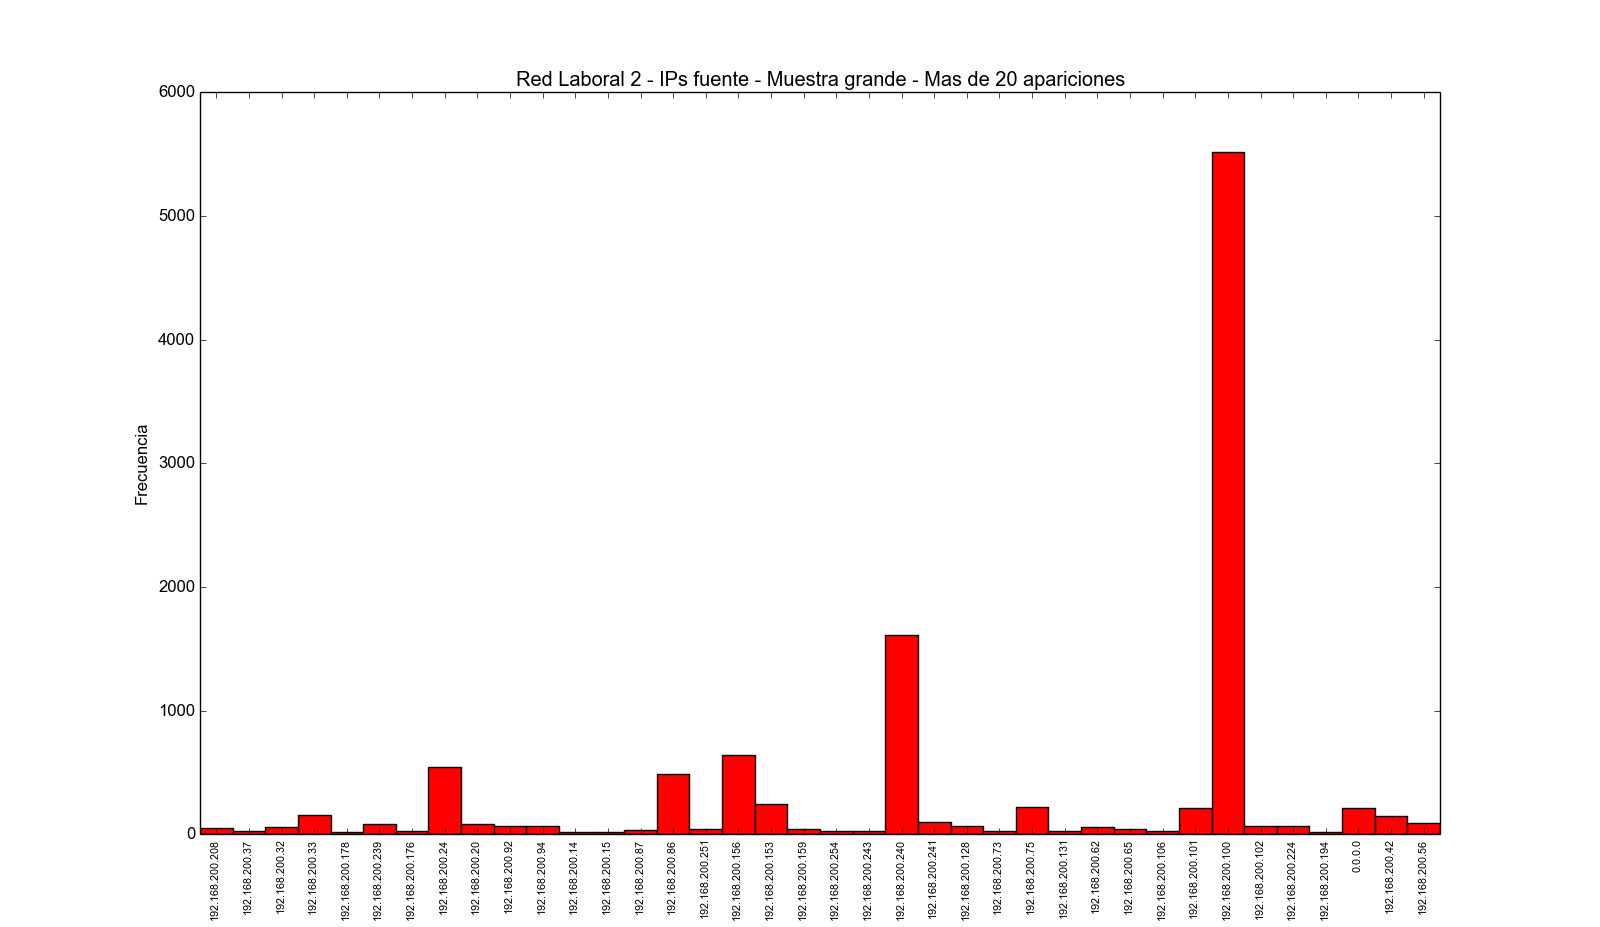
\includegraphics[scale=0.5,clip=true,trim=140 0 0 0]{graphics/laburo_src.png}

\indent Se puede observar de nuevo la predominancia de la IP 192.168.200.100, seguida nuevamente por la 192.168.200.240, aunque ahora aparecen nuevas direcciones como la 192.168.200.156.

\indent Análogamente para la fuente destino:\\

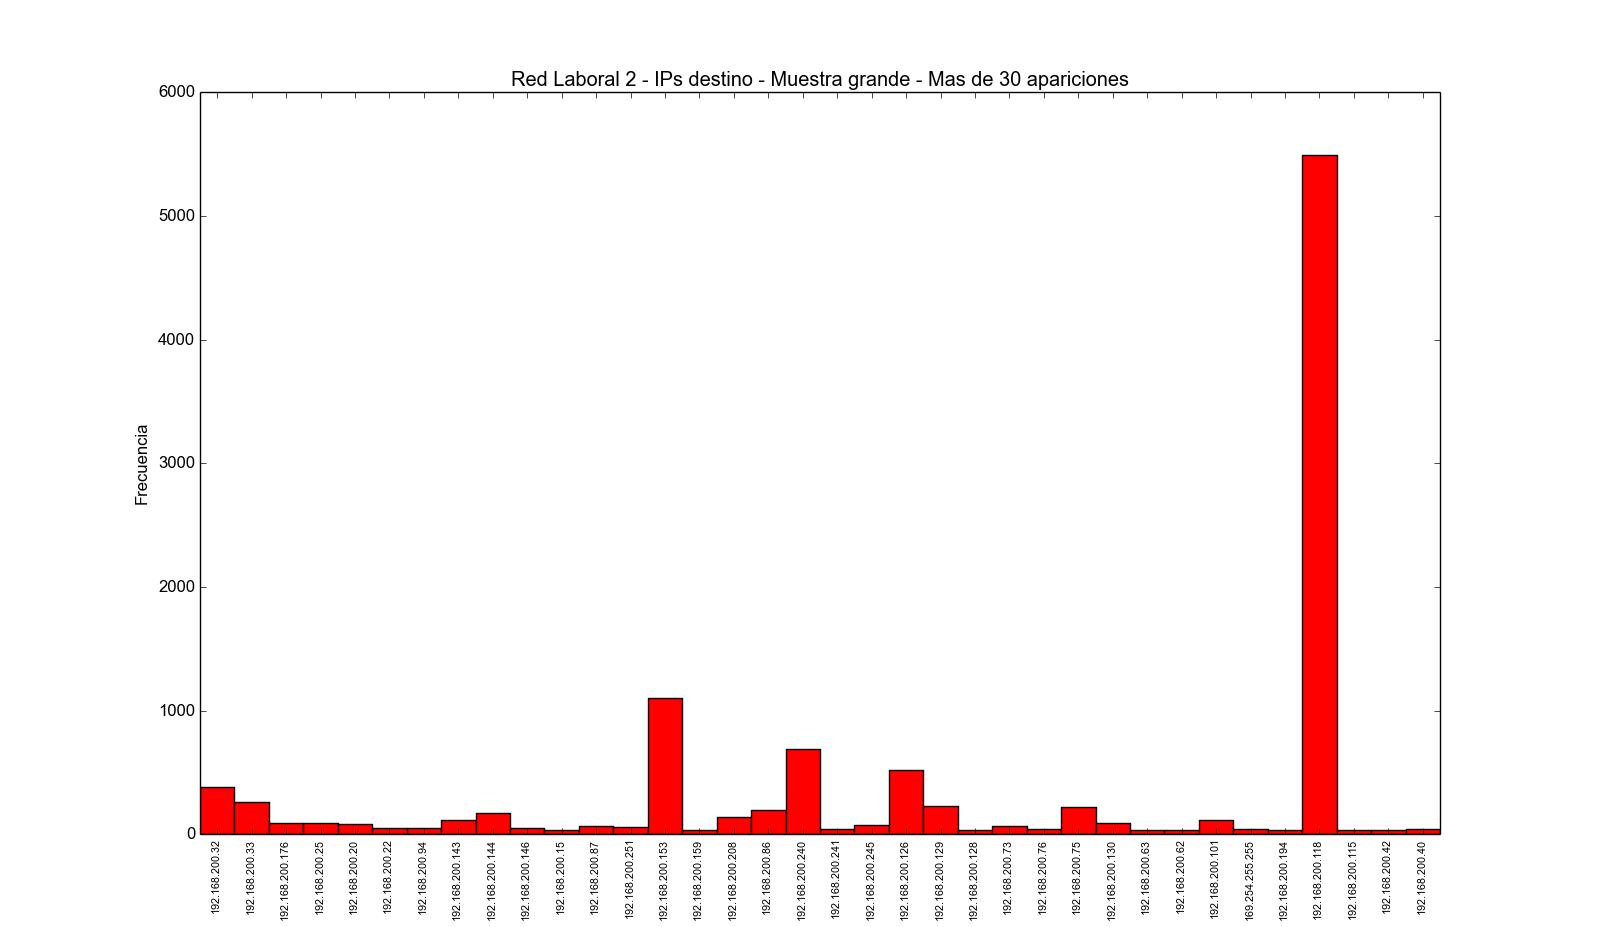
\includegraphics[scale=0.5,clip=true,trim=140 0 0 0]{graphics/laburo_dst.png}


\indent Aquí se vuelve a observar la predominancia de las IP's 192.168.200.118, 192.168.200.240 y 182.168.200.153, al igual que en los casos anteriores.\\

\indent Recordamos que debido a la gran cantidad de direcciones que entran en juego en este subcaso, no se provee un grafo de la red.\\

\indent Finalmente, los valores de entropía calculados:\\

\begin{centering}
	\begin{tabular}{ | c | c | c |} \hline
	   & \textbf{$S_{src}$} & \textbf{$S_{dst}$} \\ \hline
	  	\textbf{Entropía} & 3,6701699086665643 bits & 4,071849302811437 bits \\ \hline
	\end{tabular}
\end{centering}\\

\indent Nuevamente, creemos que los valores de entropía aumentan al incrementarse el número de direcciones que entran en juego en las capturas y que no aparecen en grandes cantidad ni en la fuente destino ni en la origen, aportando, cuando aparecen un gran valor de información.\\


\subsubsection{Sobre las direcciones 192.168.200.153 y 192.168.200.240}

\indent Teniendo conocimiento del ámbito dónde se realizó la captura, creemos que una de las dos direcciones, la 192.168.200.240, se corresponde con un router o simil, puesto que no sólo es recipiente de gran cantidad de pedidos sino que también envía muchas respuestas.\\
\indent Creemos que la dirección 192.168.200.153 se corresponde con un servidor local que se utiliza en el ámbito laboral y donde se aloja un motor de base de datos que se utiliza constantemente con las labores de Software Factory de la empresa, tanto en las áreas de desarrollo como de testeo.\\